\documentclass[twoside]{book}

% Packages required by doxygen
\usepackage{fixltx2e}
\usepackage{calc}
\usepackage{doxygen}
\usepackage[export]{adjustbox} % also loads graphicx
\usepackage{graphicx}
\usepackage[utf8]{inputenc}
\usepackage{makeidx}
\usepackage{multicol}
\usepackage{multirow}
\PassOptionsToPackage{warn}{textcomp}
\usepackage{textcomp}
\usepackage[nointegrals]{wasysym}
\usepackage[table]{xcolor}

% Font selection
\usepackage[T1]{fontenc}
\usepackage[scaled=.90]{helvet}
\usepackage{courier}
\usepackage{amssymb}
\usepackage{sectsty}
\renewcommand{\familydefault}{\sfdefault}
\allsectionsfont{%
  \fontseries{bc}\selectfont%
  \color{darkgray}%
}
\renewcommand{\DoxyLabelFont}{%
  \fontseries{bc}\selectfont%
  \color{darkgray}%
}
\newcommand{\+}{\discretionary{\mbox{\scriptsize$\hookleftarrow$}}{}{}}

% Page & text layout
\usepackage{geometry}
\geometry{%
  a4paper,%
  top=2.5cm,%
  bottom=2.5cm,%
  left=2.5cm,%
  right=2.5cm%
}
\tolerance=750
\hfuzz=15pt
\hbadness=750
\setlength{\emergencystretch}{15pt}
\setlength{\parindent}{0cm}
\setlength{\parskip}{3ex plus 2ex minus 2ex}
\makeatletter
\renewcommand{\paragraph}{%
  \@startsection{paragraph}{4}{0ex}{-1.0ex}{1.0ex}{%
    \normalfont\normalsize\bfseries\SS@parafont%
  }%
}
\renewcommand{\subparagraph}{%
  \@startsection{subparagraph}{5}{0ex}{-1.0ex}{1.0ex}{%
    \normalfont\normalsize\bfseries\SS@subparafont%
  }%
}
\makeatother

% Headers & footers
\usepackage{fancyhdr}
\pagestyle{fancyplain}
\fancyhead[LE]{\fancyplain{}{\bfseries\thepage}}
\fancyhead[CE]{\fancyplain{}{}}
\fancyhead[RE]{\fancyplain{}{\bfseries\leftmark}}
\fancyhead[LO]{\fancyplain{}{\bfseries\rightmark}}
\fancyhead[CO]{\fancyplain{}{}}
\fancyhead[RO]{\fancyplain{}{\bfseries\thepage}}
\fancyfoot[LE]{\fancyplain{}{}}
\fancyfoot[CE]{\fancyplain{}{}}
\fancyfoot[RE]{\fancyplain{}{\bfseries\scriptsize Generated by Doxygen }}
\fancyfoot[LO]{\fancyplain{}{\bfseries\scriptsize Generated by Doxygen }}
\fancyfoot[CO]{\fancyplain{}{}}
\fancyfoot[RO]{\fancyplain{}{}}
\renewcommand{\footrulewidth}{0.4pt}
\renewcommand{\chaptermark}[1]{%
  \markboth{#1}{}%
}
\renewcommand{\sectionmark}[1]{%
  \markright{\thesection\ #1}%
}

% Indices & bibliography
\usepackage{natbib}
\usepackage[titles]{tocloft}
\setcounter{tocdepth}{3}
\setcounter{secnumdepth}{5}
\makeindex

% Hyperlinks (required, but should be loaded last)
\usepackage{ifpdf}
\ifpdf
  \usepackage[pdftex,pagebackref=true]{hyperref}
\else
  \usepackage[ps2pdf,pagebackref=true]{hyperref}
\fi
\hypersetup{%
  colorlinks=true,%
  linkcolor=blue,%
  citecolor=blue,%
  unicode%
}

% Custom commands
\newcommand{\clearemptydoublepage}{%
  \newpage{\pagestyle{empty}\cleardoublepage}%
}

\usepackage{caption}
\captionsetup{labelsep=space,justification=centering,font={bf},singlelinecheck=off,skip=4pt,position=top}

%===== C O N T E N T S =====

\begin{document}

% Titlepage & ToC
\hypersetup{pageanchor=false,
             bookmarksnumbered=true,
             pdfencoding=unicode
            }
\pagenumbering{alph}
\begin{titlepage}
\vspace*{7cm}
\begin{center}%
{\Large P\+I\+C32 Boot\+Loader }\\
\vspace*{1cm}
{\large Generated by Doxygen 1.8.12}\\
\end{center}
\end{titlepage}
\clearemptydoublepage
\pagenumbering{roman}
\tableofcontents
\clearemptydoublepage
\pagenumbering{arabic}
\hypersetup{pageanchor=true}

%--- Begin generated contents ---
\chapter{File Index}
\section{File List}
Here is a list of all documented files with brief descriptions\+:\begin{DoxyCompactList}
\item\contentsline{section}{H\+:/\+Blt\+P\+I\+C32\+\_\+\+Bootloader.\+X/\hyperlink{_flash_driver_8h}{Flash\+Driver.\+h} \\*File contains the declaration of flash functions }{\pageref{_flash_driver_8h}}{}
\item\contentsline{section}{H\+:/\+Blt\+P\+I\+C32\+\_\+\+Bootloader.\+X/\hyperlink{main_8c}{main.\+c} \\*In this file the functions are defined and processed the commands from the host }{\pageref{main_8c}}{}
\item\contentsline{section}{H\+:/\+Blt\+P\+I\+C32\+\_\+\+Bootloader.\+X/\hyperlink{system_8h}{system.\+h} \\*The functions are declared and defined state enumerations }{\pageref{system_8h}}{}
\item\contentsline{section}{H\+:/\+Blt\+P\+I\+C32\+\_\+\+Bootloader.\+X/\hyperlink{_u_a_r_t_driver_8c}{U\+A\+R\+T\+Driver.\+c} \\*In this file the U\+A\+RT config, send\+Data, I\+SR functions are defined }{\pageref{_u_a_r_t_driver_8c}}{}
\item\contentsline{section}{H\+:/\+Blt\+P\+I\+C32\+\_\+\+Bootloader.\+X/\hyperlink{_u_a_r_t_driver_8h}{U\+A\+R\+T\+Driver.\+h} \\*File contains the declaration of U\+A\+RT functions and uart\+\_\+rxbuffer array }{\pageref{_u_a_r_t_driver_8h}}{}
\end{DoxyCompactList}

\chapter{File Documentation}
\hypertarget{_flash_driver_8h}{}\section{H\+:/\+Blt\+P\+I\+C32\+\_\+\+Bootloader.X/\+Flash\+Driver.h File Reference}
\label{_flash_driver_8h}\index{H\+:/\+Blt\+P\+I\+C32\+\_\+\+Bootloader.\+X/\+Flash\+Driver.\+h@{H\+:/\+Blt\+P\+I\+C32\+\_\+\+Bootloader.\+X/\+Flash\+Driver.\+h}}


File contains the declaration of flash functions.  


{\ttfamily \#include \char`\"{}system.\+h\char`\"{}}\newline
Include dependency graph for Flash\+Driver.\+h\+:
\nopagebreak
\begin{figure}[H]
\begin{center}
\leavevmode
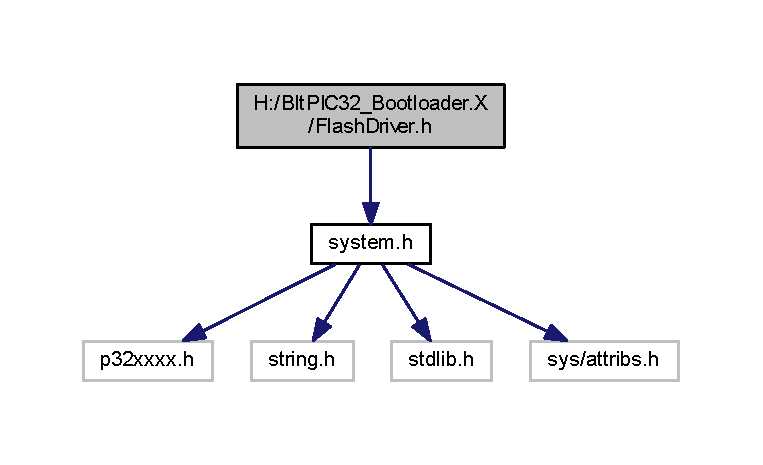
\includegraphics[width=350pt]{_flash_driver_8h__incl}
\end{center}
\end{figure}
This graph shows which files directly or indirectly include this file\+:
\nopagebreak
\begin{figure}[H]
\begin{center}
\leavevmode
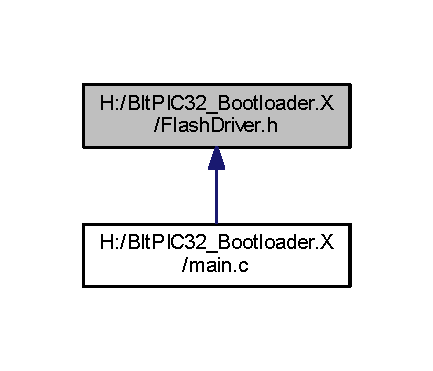
\includegraphics[width=208pt]{_flash_driver_8h__dep__incl}
\end{center}
\end{figure}
\subsection*{Macros}
\begin{DoxyCompactItemize}
\item 
\hypertarget{_flash_driver_8h_a50c7502f90d7f0662d2c725fe5d97b32}{}\label{_flash_driver_8h_a50c7502f90d7f0662d2c725fe5d97b32} 
\#define {\bfseries N\+V\+M\+O\+P\+\_\+\+W\+O\+R\+D\+\_\+\+P\+GM}~0x4001
\item 
\hypertarget{_flash_driver_8h_a416800360d5d95648dd820efc2664147}{}\label{_flash_driver_8h_a416800360d5d95648dd820efc2664147} 
\#define {\bfseries N\+V\+M\+O\+P\+\_\+\+P\+A\+G\+E\+\_\+\+E\+R\+A\+SE}~0x4004
\item 
\hypertarget{_flash_driver_8h_a78462d59d79d93ead544cc01bc8ebfdd}{}\label{_flash_driver_8h_a78462d59d79d93ead544cc01bc8ebfdd} 
\#define {\bfseries N\+V\+M\+O\+P\+\_\+\+R\+O\+W\+\_\+\+P\+GM}~0x4003
\item 
\hypertarget{_flash_driver_8h_a97d62be26684a84da173ff9374335bcc}{}\label{_flash_driver_8h_a97d62be26684a84da173ff9374335bcc} 
\#define {\bfseries N\+V\+M\+O\+P\+\_\+\+N\+OP}~0x4000
\item 
\hypertarget{_flash_driver_8h_a0c620ed67aa11b3aff9ed1ba06881f57}{}\label{_flash_driver_8h_a0c620ed67aa11b3aff9ed1ba06881f57} 
\#define {\bfseries A\+P\+P\+\_\+\+F\+L\+A\+S\+H\+\_\+\+M\+A\+X\+\_\+\+S\+I\+ZE}~(\hyperlink{system_8h_ae1fe38ff68cf2a6c82c79ef4d9b859d5}{A\+P\+P\+\_\+\+F\+L\+A\+S\+H\+\_\+\+E\+N\+D\+\_\+\+A\+D\+D\+R\+ES} -\/ \hyperlink{system_8h_a7870bb2cfb0fd58d204e2f28c9642c56}{A\+P\+P\+\_\+\+F\+L\+A\+S\+H\+\_\+\+B\+A\+S\+E\+\_\+\+A\+D\+D\+R\+E\+SS} + 1)
\item 
\hypertarget{_flash_driver_8h_a54ca0f29e0952e19933b095a7f64834f}{}\label{_flash_driver_8h_a54ca0f29e0952e19933b095a7f64834f} 
\#define {\bfseries U\+S\+E\+R\+\_\+\+A\+P\+P\+\_\+\+R\+E\+S\+E\+T\+\_\+\+A\+D\+D\+R\+E\+SS}~(0x9d006000 + 0x1000 + 0x970)
\end{DoxyCompactItemize}
\subsection*{Functions}
\begin{DoxyCompactItemize}
\item 
void \hyperlink{_flash_driver_8h_a1e791257ccfd43de12d49c29689486c2}{update\+Firmware\+\_\+\+\_\+\+Flash} (void)
\item 
void \hyperlink{_flash_driver_8h_a4e1dcc221c3ea2da41aaa12dba9d86fe}{erase\+Seq\+\_\+\+\_\+\+Flash} (void)
\end{DoxyCompactItemize}


\subsection{Detailed Description}
File contains the declaration of flash functions. 

\begin{DoxyAuthor}{Author}
Mallikarjun Tirlapur 
\end{DoxyAuthor}
\begin{DoxyDate}{Date}
16 May, 2016 
\end{DoxyDate}


\subsection{Function Documentation}
\hypertarget{_flash_driver_8h_a4e1dcc221c3ea2da41aaa12dba9d86fe}{}\label{_flash_driver_8h_a4e1dcc221c3ea2da41aaa12dba9d86fe} 
\index{Flash\+Driver.\+h@{Flash\+Driver.\+h}!erase\+Seq\+\_\+\+\_\+\+Flash@{erase\+Seq\+\_\+\+\_\+\+Flash}}
\index{erase\+Seq\+\_\+\+\_\+\+Flash@{erase\+Seq\+\_\+\+\_\+\+Flash}!Flash\+Driver.\+h@{Flash\+Driver.\+h}}
\subsubsection{\texorpdfstring{erase\+Seq\+\_\+\+\_\+\+Flash()}{eraseSeq\_\_Flash()}}
{\footnotesize\ttfamily void erase\+Seq\+\_\+\+\_\+\+Flash (\begin{DoxyParamCaption}\item[{void}]{ }\end{DoxyParamCaption})}

\begin{DoxyReturn}{Returns}

\end{DoxyReturn}
\hypertarget{_flash_driver_8h_a1e791257ccfd43de12d49c29689486c2}{}\label{_flash_driver_8h_a1e791257ccfd43de12d49c29689486c2} 
\index{Flash\+Driver.\+h@{Flash\+Driver.\+h}!update\+Firmware\+\_\+\+\_\+\+Flash@{update\+Firmware\+\_\+\+\_\+\+Flash}}
\index{update\+Firmware\+\_\+\+\_\+\+Flash@{update\+Firmware\+\_\+\+\_\+\+Flash}!Flash\+Driver.\+h@{Flash\+Driver.\+h}}
\subsubsection{\texorpdfstring{update\+Firmware\+\_\+\+\_\+\+Flash()}{updateFirmware\_\_Flash()}}
{\footnotesize\ttfamily void update\+Firmware\+\_\+\+\_\+\+Flash (\begin{DoxyParamCaption}\item[{void}]{ }\end{DoxyParamCaption})}

\begin{DoxyReturn}{Returns}

\end{DoxyReturn}

\hypertarget{main_8c}{}\section{H\+:/\+Blt\+P\+I\+C32\+\_\+\+Bootloader.X/main.c File Reference}
\label{main_8c}\index{H\+:/\+Blt\+P\+I\+C32\+\_\+\+Bootloader.\+X/main.\+c@{H\+:/\+Blt\+P\+I\+C32\+\_\+\+Bootloader.\+X/main.\+c}}


In this file the functions are defined and processed the commands from the host.  


{\ttfamily \#include \char`\"{}system.\+h\char`\"{}}\newline
{\ttfamily \#include \char`\"{}Flash\+Driver.\+h\char`\"{}}\newline
{\ttfamily \#include \char`\"{}U\+A\+R\+T\+Driver.\+h\char`\"{}}\newline
Include dependency graph for main.\+c\+:
\nopagebreak
\begin{figure}[H]
\begin{center}
\leavevmode
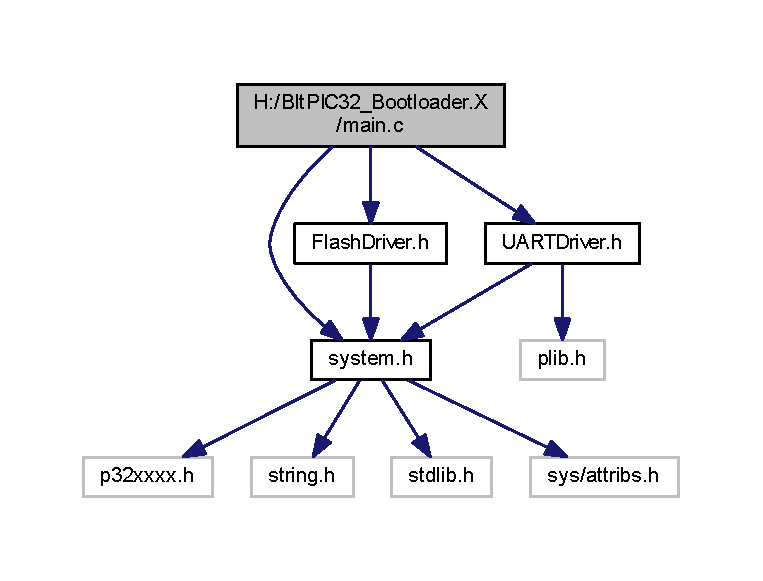
\includegraphics[width=350pt]{main_8c__incl}
\end{center}
\end{figure}
\subsection*{Functions}
\begin{DoxyCompactItemize}
\item 
\hypertarget{main_8c_a6288eba0f8e8ad3ab1544ad731eb7667}{}\label{main_8c_a6288eba0f8e8ad3ab1544ad731eb7667} 
void {\bfseries main} (void)
\item 
\hypertarget{main_8c_a41c1c05b540f333971c28ecc6647f6bf}{}\label{main_8c_a41c1c05b540f333971c28ecc6647f6bf} 
void {\bfseries init\+Var\+Config\+Port} (void)
\item 
\hypertarget{main_8c_aff608729dd08ccd2030f4e7409f857ae}{}\label{main_8c_aff608729dd08ccd2030f4e7409f857ae} 
void \hyperlink{main_8c_aff608729dd08ccd2030f4e7409f857ae}{run\+Applcn} (void)
\begin{DoxyCompactList}\small\item\em PC is updated with the new pointer to execute loaded binary from the application flash program memory. \end{DoxyCompactList}\item 
\hypertarget{main_8c_acc7a9b94b14972e9517cd0454254d16a}{}\label{main_8c_acc7a9b94b14972e9517cd0454254d16a} 
void \hyperlink{main_8c_acc7a9b94b14972e9517cd0454254d16a}{run\+State\+Machine} (void)
\begin{DoxyCompactList}\small\item\em function executes different states of the system. S\+Y\+S\+\_\+\+S\+N\+D\+\_\+\+A\+D\+D\+R\+S\+\_\+\+R\+A\+N\+GE -\/ Send the P\+IC programmable start and end address of the program memory S\+Y\+S\+\_\+\+W\+A\+I\+T\+\_\+\+F\+O\+R\+\_\+\+S\+T\+A\+R\+T\+\_\+\+C\+M\+ND -\/ The Start command triggers system to start the process and initializes buffer counter S\+Y\+S\+\_\+\+R\+C\+V\+\_\+\+F\+I\+R\+M\+W\+A\+R\+E\+\_\+\+H\+E\+A\+D\+ER -\/ Get the total packet count from the host and applcn start address S\+Y\+S\+\_\+\+C\+O\+N\+F\+I\+G\+\_\+\+F\+L\+A\+SH -\/ Erase application program area and update table pointer S\+Y\+S\+\_\+\+F\+I\+R\+M\+W\+A\+R\+E\+\_\+\+U\+P\+D\+A\+TE -\/ Receive and put the binary chunks in the flash memory S\+Y\+S\+\_\+\+R\+U\+N\+\_\+\+A\+P\+P\+L\+CN -\/ Run the application \end{DoxyCompactList}\end{DoxyCompactItemize}
\subsection*{Variables}
\begin{DoxyCompactItemize}
\item 
uint16\+\_\+t {\bfseries prog\+Mem\+Range} \mbox{[}$\,$\mbox{]}
\end{DoxyCompactItemize}


\subsection{Detailed Description}
In this file the functions are defined and processed the commands from the host. 

\begin{DoxyAuthor}{Author}
Mallikarjun Tirlapur 
\end{DoxyAuthor}
\begin{DoxyDate}{Date}
29 Aug, 2016, 11\+:04 PM 
\end{DoxyDate}


\subsection{Variable Documentation}
\hypertarget{main_8c_ad202d167fac6d1b9168605966aff3baf}{}\label{main_8c_ad202d167fac6d1b9168605966aff3baf} 
\index{main.\+c@{main.\+c}!prog\+Mem\+Range@{prog\+Mem\+Range}}
\index{prog\+Mem\+Range@{prog\+Mem\+Range}!main.\+c@{main.\+c}}
\subsubsection{\texorpdfstring{prog\+Mem\+Range}{progMemRange}}
{\footnotesize\ttfamily uint16\+\_\+t prog\+Mem\+Range\mbox{[}$\,$\mbox{]}}

{\bfseries Initial value\+:}
\begin{DoxyCode}
= \{\hyperlink{system_8h_a8afcb8142e824f079a9dbd99e7e39c4caa13f109488d193a43d676706f01038cf}{SYS\_ADDRESS\_RANGE\_TAG}, BYTE\_ROW\_SIZE, 
                         (uint8\_t)((\hyperlink{system_8h_ae1fe38ff68cf2a6c82c79ef4d9b859d5}{APP\_FLASH\_END\_ADDRES} & 0xff000000) >> 24),
                         (uint8\_t)((\hyperlink{system_8h_ae1fe38ff68cf2a6c82c79ef4d9b859d5}{APP\_FLASH\_END\_ADDRES} & 0x00ff0000) >> 16),
                         (uint8\_t)((\hyperlink{system_8h_ae1fe38ff68cf2a6c82c79ef4d9b859d5}{APP\_FLASH\_END\_ADDRES} & 0x0000ff00) >> 8),
                         (uint8\_t)(\hyperlink{system_8h_ae1fe38ff68cf2a6c82c79ef4d9b859d5}{APP\_FLASH\_END\_ADDRES} & 0x000000ff),
                         (uint8\_t)((\hyperlink{system_8h_a7870bb2cfb0fd58d204e2f28c9642c56}{APP\_FLASH\_BASE\_ADDRESS} & 0xff000000) >> 24),
                         (uint8\_t)((\hyperlink{system_8h_a7870bb2cfb0fd58d204e2f28c9642c56}{APP\_FLASH\_BASE\_ADDRESS} & 0x00ff0000) >> 16),
                         (uint8\_t)((\hyperlink{system_8h_a7870bb2cfb0fd58d204e2f28c9642c56}{APP\_FLASH\_BASE\_ADDRESS} & 0x0000ff00) >> 8),
                         (uint8\_t)(\hyperlink{system_8h_a7870bb2cfb0fd58d204e2f28c9642c56}{APP\_FLASH\_BASE\_ADDRESS} & 0x000000ff)\}
\end{DoxyCode}

\hypertarget{system_8h}{}\section{H\+:/\+Blt\+P\+I\+C32\+\_\+\+Bootloader.X/system.h File Reference}
\label{system_8h}\index{H\+:/\+Blt\+P\+I\+C32\+\_\+\+Bootloader.\+X/system.\+h@{H\+:/\+Blt\+P\+I\+C32\+\_\+\+Bootloader.\+X/system.\+h}}


The functions are declared and defined state enumerations.  


{\ttfamily \#include $<$p32xxxx.\+h$>$}\newline
{\ttfamily \#include $<$string.\+h$>$}\newline
{\ttfamily \#include $<$stdlib.\+h$>$}\newline
{\ttfamily \#include $<$sys/attribs.\+h$>$}\newline
Include dependency graph for system.\+h\+:
\nopagebreak
\begin{figure}[H]
\begin{center}
\leavevmode
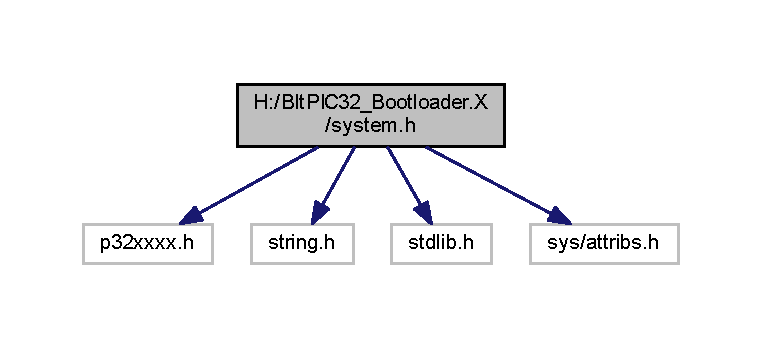
\includegraphics[width=350pt]{system_8h__incl}
\end{center}
\end{figure}
This graph shows which files directly or indirectly include this file\+:
\nopagebreak
\begin{figure}[H]
\begin{center}
\leavevmode
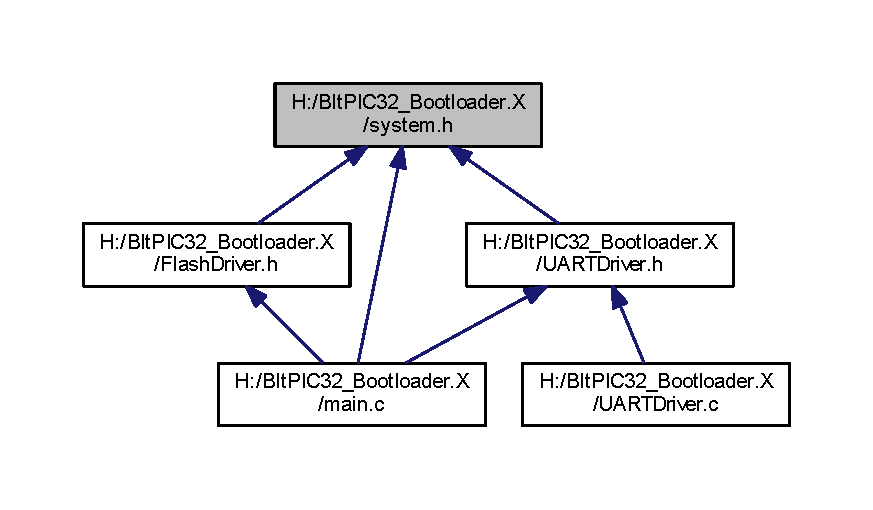
\includegraphics[width=350pt]{system_8h__dep__incl}
\end{center}
\end{figure}
\subsection*{Macros}
\begin{DoxyCompactItemize}
\item 
\hypertarget{system_8h_a08c4178cfbc31aaa81efee5588c5c6e6}{}\label{system_8h_a08c4178cfbc31aaa81efee5588c5c6e6} 
\#define {\bfseries N\+V\+M\+\_\+\+P\+A\+G\+E\+\_\+\+S\+I\+ZE}~1024
\item 
\hypertarget{system_8h_a66af65341db20a62c99c70dc9928a18f}{}\label{system_8h_a66af65341db20a62c99c70dc9928a18f} 
\#define {\bfseries B\+Y\+T\+E\+\_\+\+P\+A\+G\+E\+\_\+\+S\+I\+ZE}~(4 $\ast$ P\+A\+G\+E\+\_\+\+S\+I\+ZE)
\item 
\hypertarget{system_8h_aa4d030604a90c8d019d90fc721900d63}{}\label{system_8h_aa4d030604a90c8d019d90fc721900d63} 
\#define {\bfseries R\+O\+W\+\_\+\+S\+I\+ZE}~128
\item 
\hypertarget{system_8h_a66585fa14329bd6cbb93c0d1a8964658}{}\label{system_8h_a66585fa14329bd6cbb93c0d1a8964658} 
\#define {\bfseries B\+Y\+T\+E\+\_\+\+R\+O\+W\+\_\+\+S\+I\+ZE}~(4 $\ast$ R\+O\+W\+\_\+\+S\+I\+ZE)
\item 
\hypertarget{system_8h_a38aa50b0a3c01e2f2f0d6917a548c74b}{}\label{system_8h_a38aa50b0a3c01e2f2f0d6917a548c74b} 
\#define {\bfseries N\+U\+M\+\_\+\+R\+O\+W\+S\+\_\+\+P\+A\+GE}~8
\item 
\#define \hyperlink{system_8h_a7870bb2cfb0fd58d204e2f28c9642c56}{A\+P\+P\+\_\+\+F\+L\+A\+S\+H\+\_\+\+B\+A\+S\+E\+\_\+\+A\+D\+D\+R\+E\+SS}~0x9\+D006000
\item 
\#define \hyperlink{system_8h_ae1fe38ff68cf2a6c82c79ef4d9b859d5}{A\+P\+P\+\_\+\+F\+L\+A\+S\+H\+\_\+\+E\+N\+D\+\_\+\+A\+D\+D\+R\+ES}~0x9\+D00\+F\+F\+FF
\end{DoxyCompactItemize}
\subsection*{Typedefs}
\begin{DoxyCompactItemize}
\item 
\hypertarget{system_8h_aba7bc1797add20fe3efdf37ced1182c5}{}\label{system_8h_aba7bc1797add20fe3efdf37ced1182c5} 
typedef unsigned char {\bfseries uint8\+\_\+t}
\item 
\hypertarget{system_8h_a273cf69d639a59973b6019625df33e30}{}\label{system_8h_a273cf69d639a59973b6019625df33e30} 
typedef unsigned short {\bfseries uint16\+\_\+t}
\item 
\hypertarget{system_8h_a06896e8c53f721507066c079052171f8}{}\label{system_8h_a06896e8c53f721507066c079052171f8} 
typedef unsigned long {\bfseries uint32\+\_\+t}
\item 
\hypertarget{system_8h_a12a1e9b3ce141648783a82445d02b58d}{}\label{system_8h_a12a1e9b3ce141648783a82445d02b58d} 
typedef unsigned int {\bfseries uint\+\_\+t}
\item 
\hypertarget{system_8h_a80a6557a4ef72cc3c9097c5d9bf9aa1e}{}\label{system_8h_a80a6557a4ef72cc3c9097c5d9bf9aa1e} 
typedef enum \hyperlink{system_8h_a2b9e977e16660cb036853d1ab4bf4a4d}{S\+Y\+S\+T\+E\+M\+\_\+\+S\+T\+A\+T\+U\+S\+\_\+\+Tag} \hyperlink{system_8h_a80a6557a4ef72cc3c9097c5d9bf9aa1e}{S\+Y\+S\+\_\+\+S\+T\+A\+T\+E\+\_\+t}
\begin{DoxyCompactList}\small\item\em Enumeral represents different system states. \end{DoxyCompactList}\item 
\hypertarget{system_8h_acc42fa44351dc534575acae91880e834}{}\label{system_8h_acc42fa44351dc534575acae91880e834} 
typedef enum \hyperlink{system_8h_a8afcb8142e824f079a9dbd99e7e39c4c}{S\+Y\+S\+T\+E\+M\+\_\+\+C\+O\+M\+\_\+\+P\+R\+O\+T\+O\+C\+O\+L\+\_\+\+M\+S\+G\+\_\+\+Tag} \hyperlink{system_8h_acc42fa44351dc534575acae91880e834}{S\+Y\+S\+\_\+\+C\+O\+M\+\_\+\+P\+R\+O\+T\+O\+C\+L\+\_\+\+M\+S\+G\+\_\+t}
\begin{DoxyCompactList}\small\item\em Enumeral represents handshaking signals between programmer and controller. \end{DoxyCompactList}\end{DoxyCompactItemize}
\subsection*{Enumerations}
\begin{DoxyCompactItemize}
\item 
enum \hyperlink{system_8h_a2b9e977e16660cb036853d1ab4bf4a4d}{S\+Y\+S\+T\+E\+M\+\_\+\+S\+T\+A\+T\+U\+S\+\_\+\+Tag} \{ \newline
\hyperlink{system_8h_a2b9e977e16660cb036853d1ab4bf4a4da9e627365054b4d0d176a65b4452ec1d2}{S\+Y\+S\+\_\+\+W\+A\+I\+T\+\_\+\+F\+O\+R\+\_\+\+S\+T\+A\+R\+T\+\_\+\+C\+M\+ND}, 
\hyperlink{system_8h_a2b9e977e16660cb036853d1ab4bf4a4da95bd289c0c68a6ae62dfbd787d4a4fa2}{S\+Y\+S\+\_\+\+C\+O\+N\+F\+I\+G\+\_\+\+F\+L\+A\+SH}, 
\hyperlink{system_8h_a2b9e977e16660cb036853d1ab4bf4a4da72674f33fcdaba13529ebe41f00494c9}{S\+Y\+S\+\_\+\+R\+C\+V\+\_\+\+F\+I\+R\+M\+W\+A\+R\+E\+\_\+\+H\+E\+A\+D\+ER}, 
\hyperlink{system_8h_a2b9e977e16660cb036853d1ab4bf4a4da7db56bbca7269565ec45dcc81ccdf419}{S\+Y\+S\+\_\+\+F\+I\+R\+M\+W\+A\+R\+E\+\_\+\+U\+P\+D\+A\+TE}, 
\newline
\hyperlink{system_8h_a2b9e977e16660cb036853d1ab4bf4a4daa303948971c6fed2bcb3f62e7606d3f9}{S\+Y\+S\+\_\+\+R\+U\+N\+\_\+\+A\+P\+P\+L\+CN}, 
\hyperlink{system_8h_a2b9e977e16660cb036853d1ab4bf4a4dabcd03ff568b9283ad95e36da773be1d8}{S\+Y\+S\+\_\+\+S\+N\+D\+\_\+\+A\+D\+D\+R\+S\+\_\+\+R\+A\+N\+GE}
 \}\begin{DoxyCompactList}\small\item\em Enumeral represents different system states. \end{DoxyCompactList}
\item 
enum \hyperlink{system_8h_a8afcb8142e824f079a9dbd99e7e39c4c}{S\+Y\+S\+T\+E\+M\+\_\+\+C\+O\+M\+\_\+\+P\+R\+O\+T\+O\+C\+O\+L\+\_\+\+M\+S\+G\+\_\+\+Tag} \{ \newline
\hyperlink{system_8h_a8afcb8142e824f079a9dbd99e7e39c4cad0ae523c145748b0787c7245968e24a6}{S\+Y\+S\+\_\+\+S\+T\+A\+R\+T\+\_\+\+C\+M\+N\+D\+\_\+\+F\+R\+O\+M\+\_\+\+P\+R\+O\+G\+R\+MR} = 0x01, 
\hyperlink{system_8h_a8afcb8142e824f079a9dbd99e7e39c4ca06807f76d857573262e70814425e79dd}{S\+Y\+S\+\_\+\+R\+E\+A\+D\+Y\+\_\+\+F\+O\+R\+\_\+\+F\+I\+R\+M\+W\+A\+R\+E\+\_\+\+H\+E\+A\+D\+ER}, 
\hyperlink{system_8h_a8afcb8142e824f079a9dbd99e7e39c4cad6d077f54204532926ab5c91ca00858b}{S\+Y\+S\+\_\+\+F\+I\+R\+M\+W\+A\+R\+E\+\_\+\+H\+E\+A\+D\+E\+R\+\_\+\+P\+O\+S\+\_\+\+A\+CK}, 
\hyperlink{system_8h_a8afcb8142e824f079a9dbd99e7e39c4ca5c5902b8a5a56c9fb0ef28c30f4d5e09}{S\+Y\+S\+\_\+\+F\+I\+R\+M\+W\+A\+R\+E\+\_\+\+H\+E\+A\+D\+E\+R\+\_\+\+N\+E\+G\+\_\+\+A\+CK}, 
\newline
\hyperlink{system_8h_a8afcb8142e824f079a9dbd99e7e39c4ca568d188ecdf4fb8f56eb9c133eae645d}{S\+Y\+S\+\_\+\+S\+N\+D\+\_\+\+N\+X\+T\+\_\+\+C\+H\+U\+NK}, 
\hyperlink{system_8h_a8afcb8142e824f079a9dbd99e7e39c4caa13f109488d193a43d676706f01038cf}{S\+Y\+S\+\_\+\+A\+D\+D\+R\+E\+S\+S\+\_\+\+R\+A\+N\+G\+E\+\_\+\+T\+AG}, 
\hyperlink{system_8h_a8afcb8142e824f079a9dbd99e7e39c4cac839497a309b7e91de9b8356cde9ea95}{S\+Y\+S\+\_\+\+A\+D\+D\+R\+E\+S\+S\+\_\+\+R\+A\+N\+G\+E\+\_\+\+R\+QT}
 \}\begin{DoxyCompactList}\small\item\em Enumeral represents handshaking signals between programmer and controller. \end{DoxyCompactList}
\end{DoxyCompactItemize}
\subsection*{Functions}
\begin{DoxyCompactItemize}
\item 
\hypertarget{system_8h_acc7a9b94b14972e9517cd0454254d16a}{}\label{system_8h_acc7a9b94b14972e9517cd0454254d16a} 
void \hyperlink{system_8h_acc7a9b94b14972e9517cd0454254d16a}{run\+State\+Machine} (void)
\begin{DoxyCompactList}\small\item\em function executes different states of the system. S\+Y\+S\+\_\+\+S\+N\+D\+\_\+\+A\+D\+D\+R\+S\+\_\+\+R\+A\+N\+GE -\/ Send the P\+IC programmable start and end address of the program memory S\+Y\+S\+\_\+\+W\+A\+I\+T\+\_\+\+F\+O\+R\+\_\+\+S\+T\+A\+R\+T\+\_\+\+C\+M\+ND -\/ The Start command triggers system to start the process and initializes buffer counter S\+Y\+S\+\_\+\+R\+C\+V\+\_\+\+F\+I\+R\+M\+W\+A\+R\+E\+\_\+\+H\+E\+A\+D\+ER -\/ Get the total packet count from the host and applcn start address S\+Y\+S\+\_\+\+C\+O\+N\+F\+I\+G\+\_\+\+F\+L\+A\+SH -\/ Erase application program area and update table pointer S\+Y\+S\+\_\+\+F\+I\+R\+M\+W\+A\+R\+E\+\_\+\+U\+P\+D\+A\+TE -\/ Receive and put the binary chunks in the flash memory S\+Y\+S\+\_\+\+R\+U\+N\+\_\+\+A\+P\+P\+L\+CN -\/ Run the application \end{DoxyCompactList}\item 
\hypertarget{system_8h_a41c1c05b540f333971c28ecc6647f6bf}{}\label{system_8h_a41c1c05b540f333971c28ecc6647f6bf} 
void {\bfseries init\+Var\+Config\+Port} (void)
\item 
\hypertarget{system_8h_aff608729dd08ccd2030f4e7409f857ae}{}\label{system_8h_aff608729dd08ccd2030f4e7409f857ae} 
void \hyperlink{system_8h_aff608729dd08ccd2030f4e7409f857ae}{run\+Applcn} (void)
\begin{DoxyCompactList}\small\item\em PC is updated with the new pointer to execute loaded binary from the application flash program memory. \end{DoxyCompactList}\end{DoxyCompactItemize}
\subsection*{Variables}
\begin{DoxyCompactItemize}
\item 
uint32\+\_\+t \hyperlink{system_8h_a8624df3154717d6117c76cc95b7175de}{appl\+Start\+Add}
\item 
uint8\+\_\+t \hyperlink{system_8h_ab1afd31b449a5606fe3c15946427f29a}{total\+Number\+Of\+Pacckets}
\end{DoxyCompactItemize}


\subsection{Detailed Description}
The functions are declared and defined state enumerations. 

\begin{DoxyAuthor}{Author}
Mallikarjun Tirlapur 
\end{DoxyAuthor}
\begin{DoxyDate}{Date}
16 May, 2016 
\end{DoxyDate}


\subsection{Macro Definition Documentation}
\hypertarget{system_8h_a7870bb2cfb0fd58d204e2f28c9642c56}{}\label{system_8h_a7870bb2cfb0fd58d204e2f28c9642c56} 
\index{system.\+h@{system.\+h}!A\+P\+P\+\_\+\+F\+L\+A\+S\+H\+\_\+\+B\+A\+S\+E\+\_\+\+A\+D\+D\+R\+E\+SS@{A\+P\+P\+\_\+\+F\+L\+A\+S\+H\+\_\+\+B\+A\+S\+E\+\_\+\+A\+D\+D\+R\+E\+SS}}
\index{A\+P\+P\+\_\+\+F\+L\+A\+S\+H\+\_\+\+B\+A\+S\+E\+\_\+\+A\+D\+D\+R\+E\+SS@{A\+P\+P\+\_\+\+F\+L\+A\+S\+H\+\_\+\+B\+A\+S\+E\+\_\+\+A\+D\+D\+R\+E\+SS}!system.\+h@{system.\+h}}
\subsubsection{\texorpdfstring{A\+P\+P\+\_\+\+F\+L\+A\+S\+H\+\_\+\+B\+A\+S\+E\+\_\+\+A\+D\+D\+R\+E\+SS}{APP\_FLASH\_BASE\_ADDRESS}}
{\footnotesize\ttfamily \#define A\+P\+P\+\_\+\+F\+L\+A\+S\+H\+\_\+\+B\+A\+S\+E\+\_\+\+A\+D\+D\+R\+E\+SS~0x9\+D006000}

N\+VM start adress. \hypertarget{system_8h_ae1fe38ff68cf2a6c82c79ef4d9b859d5}{}\label{system_8h_ae1fe38ff68cf2a6c82c79ef4d9b859d5} 
\index{system.\+h@{system.\+h}!A\+P\+P\+\_\+\+F\+L\+A\+S\+H\+\_\+\+E\+N\+D\+\_\+\+A\+D\+D\+R\+ES@{A\+P\+P\+\_\+\+F\+L\+A\+S\+H\+\_\+\+E\+N\+D\+\_\+\+A\+D\+D\+R\+ES}}
\index{A\+P\+P\+\_\+\+F\+L\+A\+S\+H\+\_\+\+E\+N\+D\+\_\+\+A\+D\+D\+R\+ES@{A\+P\+P\+\_\+\+F\+L\+A\+S\+H\+\_\+\+E\+N\+D\+\_\+\+A\+D\+D\+R\+ES}!system.\+h@{system.\+h}}
\subsubsection{\texorpdfstring{A\+P\+P\+\_\+\+F\+L\+A\+S\+H\+\_\+\+E\+N\+D\+\_\+\+A\+D\+D\+R\+ES}{APP\_FLASH\_END\_ADDRES}}
{\footnotesize\ttfamily \#define A\+P\+P\+\_\+\+F\+L\+A\+S\+H\+\_\+\+E\+N\+D\+\_\+\+A\+D\+D\+R\+ES~0x9\+D00\+F\+F\+FF}

N\+VM end adress. 

\subsection{Enumeration Type Documentation}
\hypertarget{system_8h_a8afcb8142e824f079a9dbd99e7e39c4c}{}\label{system_8h_a8afcb8142e824f079a9dbd99e7e39c4c} 
\index{system.\+h@{system.\+h}!S\+Y\+S\+T\+E\+M\+\_\+\+C\+O\+M\+\_\+\+P\+R\+O\+T\+O\+C\+O\+L\+\_\+\+M\+S\+G\+\_\+\+Tag@{S\+Y\+S\+T\+E\+M\+\_\+\+C\+O\+M\+\_\+\+P\+R\+O\+T\+O\+C\+O\+L\+\_\+\+M\+S\+G\+\_\+\+Tag}}
\index{S\+Y\+S\+T\+E\+M\+\_\+\+C\+O\+M\+\_\+\+P\+R\+O\+T\+O\+C\+O\+L\+\_\+\+M\+S\+G\+\_\+\+Tag@{S\+Y\+S\+T\+E\+M\+\_\+\+C\+O\+M\+\_\+\+P\+R\+O\+T\+O\+C\+O\+L\+\_\+\+M\+S\+G\+\_\+\+Tag}!system.\+h@{system.\+h}}
\subsubsection{\texorpdfstring{S\+Y\+S\+T\+E\+M\+\_\+\+C\+O\+M\+\_\+\+P\+R\+O\+T\+O\+C\+O\+L\+\_\+\+M\+S\+G\+\_\+\+Tag}{SYSTEM\_COM\_PROTOCOL\_MSG\_Tag}}
{\footnotesize\ttfamily enum \hyperlink{system_8h_a8afcb8142e824f079a9dbd99e7e39c4c}{S\+Y\+S\+T\+E\+M\+\_\+\+C\+O\+M\+\_\+\+P\+R\+O\+T\+O\+C\+O\+L\+\_\+\+M\+S\+G\+\_\+\+Tag}}



Enumeral represents handshaking signals between programmer and controller. 

\begin{DoxyEnumFields}{Enumerator}
\raisebox{\heightof{T}}[0pt][0pt]{\index{S\+Y\+S\+\_\+\+S\+T\+A\+R\+T\+\_\+\+C\+M\+N\+D\+\_\+\+F\+R\+O\+M\+\_\+\+P\+R\+O\+G\+R\+MR@{S\+Y\+S\+\_\+\+S\+T\+A\+R\+T\+\_\+\+C\+M\+N\+D\+\_\+\+F\+R\+O\+M\+\_\+\+P\+R\+O\+G\+R\+MR}!system.\+h@{system.\+h}}\index{system.\+h@{system.\+h}!S\+Y\+S\+\_\+\+S\+T\+A\+R\+T\+\_\+\+C\+M\+N\+D\+\_\+\+F\+R\+O\+M\+\_\+\+P\+R\+O\+G\+R\+MR@{S\+Y\+S\+\_\+\+S\+T\+A\+R\+T\+\_\+\+C\+M\+N\+D\+\_\+\+F\+R\+O\+M\+\_\+\+P\+R\+O\+G\+R\+MR}}}\hypertarget{system_8h_a8afcb8142e824f079a9dbd99e7e39c4cad0ae523c145748b0787c7245968e24a6}{}\label{system_8h_a8afcb8142e824f079a9dbd99e7e39c4cad0ae523c145748b0787c7245968e24a6} 
S\+Y\+S\+\_\+\+S\+T\+A\+R\+T\+\_\+\+C\+M\+N\+D\+\_\+\+F\+R\+O\+M\+\_\+\+P\+R\+O\+G\+R\+MR&Config command signal from the programmer. \\
\hline

\raisebox{\heightof{T}}[0pt][0pt]{\index{S\+Y\+S\+\_\+\+R\+E\+A\+D\+Y\+\_\+\+F\+O\+R\+\_\+\+F\+I\+R\+M\+W\+A\+R\+E\+\_\+\+H\+E\+A\+D\+ER@{S\+Y\+S\+\_\+\+R\+E\+A\+D\+Y\+\_\+\+F\+O\+R\+\_\+\+F\+I\+R\+M\+W\+A\+R\+E\+\_\+\+H\+E\+A\+D\+ER}!system.\+h@{system.\+h}}\index{system.\+h@{system.\+h}!S\+Y\+S\+\_\+\+R\+E\+A\+D\+Y\+\_\+\+F\+O\+R\+\_\+\+F\+I\+R\+M\+W\+A\+R\+E\+\_\+\+H\+E\+A\+D\+ER@{S\+Y\+S\+\_\+\+R\+E\+A\+D\+Y\+\_\+\+F\+O\+R\+\_\+\+F\+I\+R\+M\+W\+A\+R\+E\+\_\+\+H\+E\+A\+D\+ER}}}\hypertarget{system_8h_a8afcb8142e824f079a9dbd99e7e39c4ca06807f76d857573262e70814425e79dd}{}\label{system_8h_a8afcb8142e824f079a9dbd99e7e39c4ca06807f76d857573262e70814425e79dd} 
S\+Y\+S\+\_\+\+R\+E\+A\+D\+Y\+\_\+\+F\+O\+R\+\_\+\+F\+I\+R\+M\+W\+A\+R\+E\+\_\+\+H\+E\+A\+D\+ER&Ready for firmware header signal sent to the programmer. \\
\hline

\raisebox{\heightof{T}}[0pt][0pt]{\index{S\+Y\+S\+\_\+\+F\+I\+R\+M\+W\+A\+R\+E\+\_\+\+H\+E\+A\+D\+E\+R\+\_\+\+P\+O\+S\+\_\+\+A\+CK@{S\+Y\+S\+\_\+\+F\+I\+R\+M\+W\+A\+R\+E\+\_\+\+H\+E\+A\+D\+E\+R\+\_\+\+P\+O\+S\+\_\+\+A\+CK}!system.\+h@{system.\+h}}\index{system.\+h@{system.\+h}!S\+Y\+S\+\_\+\+F\+I\+R\+M\+W\+A\+R\+E\+\_\+\+H\+E\+A\+D\+E\+R\+\_\+\+P\+O\+S\+\_\+\+A\+CK@{S\+Y\+S\+\_\+\+F\+I\+R\+M\+W\+A\+R\+E\+\_\+\+H\+E\+A\+D\+E\+R\+\_\+\+P\+O\+S\+\_\+\+A\+CK}}}\hypertarget{system_8h_a8afcb8142e824f079a9dbd99e7e39c4cad6d077f54204532926ab5c91ca00858b}{}\label{system_8h_a8afcb8142e824f079a9dbd99e7e39c4cad6d077f54204532926ab5c91ca00858b} 
S\+Y\+S\+\_\+\+F\+I\+R\+M\+W\+A\+R\+E\+\_\+\+H\+E\+A\+D\+E\+R\+\_\+\+P\+O\+S\+\_\+\+A\+CK&Firmware header positive acknowledgement. \\
\hline

\raisebox{\heightof{T}}[0pt][0pt]{\index{S\+Y\+S\+\_\+\+F\+I\+R\+M\+W\+A\+R\+E\+\_\+\+H\+E\+A\+D\+E\+R\+\_\+\+N\+E\+G\+\_\+\+A\+CK@{S\+Y\+S\+\_\+\+F\+I\+R\+M\+W\+A\+R\+E\+\_\+\+H\+E\+A\+D\+E\+R\+\_\+\+N\+E\+G\+\_\+\+A\+CK}!system.\+h@{system.\+h}}\index{system.\+h@{system.\+h}!S\+Y\+S\+\_\+\+F\+I\+R\+M\+W\+A\+R\+E\+\_\+\+H\+E\+A\+D\+E\+R\+\_\+\+N\+E\+G\+\_\+\+A\+CK@{S\+Y\+S\+\_\+\+F\+I\+R\+M\+W\+A\+R\+E\+\_\+\+H\+E\+A\+D\+E\+R\+\_\+\+N\+E\+G\+\_\+\+A\+CK}}}\hypertarget{system_8h_a8afcb8142e824f079a9dbd99e7e39c4ca5c5902b8a5a56c9fb0ef28c30f4d5e09}{}\label{system_8h_a8afcb8142e824f079a9dbd99e7e39c4ca5c5902b8a5a56c9fb0ef28c30f4d5e09} 
S\+Y\+S\+\_\+\+F\+I\+R\+M\+W\+A\+R\+E\+\_\+\+H\+E\+A\+D\+E\+R\+\_\+\+N\+E\+G\+\_\+\+A\+CK&Firmware header negative acknowledgement. \\
\hline

\raisebox{\heightof{T}}[0pt][0pt]{\index{S\+Y\+S\+\_\+\+S\+N\+D\+\_\+\+N\+X\+T\+\_\+\+C\+H\+U\+NK@{S\+Y\+S\+\_\+\+S\+N\+D\+\_\+\+N\+X\+T\+\_\+\+C\+H\+U\+NK}!system.\+h@{system.\+h}}\index{system.\+h@{system.\+h}!S\+Y\+S\+\_\+\+S\+N\+D\+\_\+\+N\+X\+T\+\_\+\+C\+H\+U\+NK@{S\+Y\+S\+\_\+\+S\+N\+D\+\_\+\+N\+X\+T\+\_\+\+C\+H\+U\+NK}}}\hypertarget{system_8h_a8afcb8142e824f079a9dbd99e7e39c4ca568d188ecdf4fb8f56eb9c133eae645d}{}\label{system_8h_a8afcb8142e824f079a9dbd99e7e39c4ca568d188ecdf4fb8f56eb9c133eae645d} 
S\+Y\+S\+\_\+\+S\+N\+D\+\_\+\+N\+X\+T\+\_\+\+C\+H\+U\+NK&send next chunk signal. \\
\hline

\raisebox{\heightof{T}}[0pt][0pt]{\index{S\+Y\+S\+\_\+\+A\+D\+D\+R\+E\+S\+S\+\_\+\+R\+A\+N\+G\+E\+\_\+\+T\+AG@{S\+Y\+S\+\_\+\+A\+D\+D\+R\+E\+S\+S\+\_\+\+R\+A\+N\+G\+E\+\_\+\+T\+AG}!system.\+h@{system.\+h}}\index{system.\+h@{system.\+h}!S\+Y\+S\+\_\+\+A\+D\+D\+R\+E\+S\+S\+\_\+\+R\+A\+N\+G\+E\+\_\+\+T\+AG@{S\+Y\+S\+\_\+\+A\+D\+D\+R\+E\+S\+S\+\_\+\+R\+A\+N\+G\+E\+\_\+\+T\+AG}}}\hypertarget{system_8h_a8afcb8142e824f079a9dbd99e7e39c4caa13f109488d193a43d676706f01038cf}{}\label{system_8h_a8afcb8142e824f079a9dbd99e7e39c4caa13f109488d193a43d676706f01038cf} 
S\+Y\+S\+\_\+\+A\+D\+D\+R\+E\+S\+S\+\_\+\+R\+A\+N\+G\+E\+\_\+\+T\+AG&send address with this tag. \\
\hline

\raisebox{\heightof{T}}[0pt][0pt]{\index{S\+Y\+S\+\_\+\+A\+D\+D\+R\+E\+S\+S\+\_\+\+R\+A\+N\+G\+E\+\_\+\+R\+QT@{S\+Y\+S\+\_\+\+A\+D\+D\+R\+E\+S\+S\+\_\+\+R\+A\+N\+G\+E\+\_\+\+R\+QT}!system.\+h@{system.\+h}}\index{system.\+h@{system.\+h}!S\+Y\+S\+\_\+\+A\+D\+D\+R\+E\+S\+S\+\_\+\+R\+A\+N\+G\+E\+\_\+\+R\+QT@{S\+Y\+S\+\_\+\+A\+D\+D\+R\+E\+S\+S\+\_\+\+R\+A\+N\+G\+E\+\_\+\+R\+QT}}}\hypertarget{system_8h_a8afcb8142e824f079a9dbd99e7e39c4cac839497a309b7e91de9b8356cde9ea95}{}\label{system_8h_a8afcb8142e824f079a9dbd99e7e39c4cac839497a309b7e91de9b8356cde9ea95} 
S\+Y\+S\+\_\+\+A\+D\+D\+R\+E\+S\+S\+\_\+\+R\+A\+N\+G\+E\+\_\+\+R\+QT&Rquest for the address from the host. \\
\hline

\end{DoxyEnumFields}
\hypertarget{system_8h_a2b9e977e16660cb036853d1ab4bf4a4d}{}\label{system_8h_a2b9e977e16660cb036853d1ab4bf4a4d} 
\index{system.\+h@{system.\+h}!S\+Y\+S\+T\+E\+M\+\_\+\+S\+T\+A\+T\+U\+S\+\_\+\+Tag@{S\+Y\+S\+T\+E\+M\+\_\+\+S\+T\+A\+T\+U\+S\+\_\+\+Tag}}
\index{S\+Y\+S\+T\+E\+M\+\_\+\+S\+T\+A\+T\+U\+S\+\_\+\+Tag@{S\+Y\+S\+T\+E\+M\+\_\+\+S\+T\+A\+T\+U\+S\+\_\+\+Tag}!system.\+h@{system.\+h}}
\subsubsection{\texorpdfstring{S\+Y\+S\+T\+E\+M\+\_\+\+S\+T\+A\+T\+U\+S\+\_\+\+Tag}{SYSTEM\_STATUS\_Tag}}
{\footnotesize\ttfamily enum \hyperlink{system_8h_a2b9e977e16660cb036853d1ab4bf4a4d}{S\+Y\+S\+T\+E\+M\+\_\+\+S\+T\+A\+T\+U\+S\+\_\+\+Tag}}



Enumeral represents different system states. 

\begin{DoxyEnumFields}{Enumerator}
\raisebox{\heightof{T}}[0pt][0pt]{\index{S\+Y\+S\+\_\+\+W\+A\+I\+T\+\_\+\+F\+O\+R\+\_\+\+S\+T\+A\+R\+T\+\_\+\+C\+M\+ND@{S\+Y\+S\+\_\+\+W\+A\+I\+T\+\_\+\+F\+O\+R\+\_\+\+S\+T\+A\+R\+T\+\_\+\+C\+M\+ND}!system.\+h@{system.\+h}}\index{system.\+h@{system.\+h}!S\+Y\+S\+\_\+\+W\+A\+I\+T\+\_\+\+F\+O\+R\+\_\+\+S\+T\+A\+R\+T\+\_\+\+C\+M\+ND@{S\+Y\+S\+\_\+\+W\+A\+I\+T\+\_\+\+F\+O\+R\+\_\+\+S\+T\+A\+R\+T\+\_\+\+C\+M\+ND}}}\hypertarget{system_8h_a2b9e977e16660cb036853d1ab4bf4a4da9e627365054b4d0d176a65b4452ec1d2}{}\label{system_8h_a2b9e977e16660cb036853d1ab4bf4a4da9e627365054b4d0d176a65b4452ec1d2} 
S\+Y\+S\+\_\+\+W\+A\+I\+T\+\_\+\+F\+O\+R\+\_\+\+S\+T\+A\+R\+T\+\_\+\+C\+M\+ND&State where system waits for a start command from the programmer. \\
\hline

\raisebox{\heightof{T}}[0pt][0pt]{\index{S\+Y\+S\+\_\+\+C\+O\+N\+F\+I\+G\+\_\+\+F\+L\+A\+SH@{S\+Y\+S\+\_\+\+C\+O\+N\+F\+I\+G\+\_\+\+F\+L\+A\+SH}!system.\+h@{system.\+h}}\index{system.\+h@{system.\+h}!S\+Y\+S\+\_\+\+C\+O\+N\+F\+I\+G\+\_\+\+F\+L\+A\+SH@{S\+Y\+S\+\_\+\+C\+O\+N\+F\+I\+G\+\_\+\+F\+L\+A\+SH}}}\hypertarget{system_8h_a2b9e977e16660cb036853d1ab4bf4a4da95bd289c0c68a6ae62dfbd787d4a4fa2}{}\label{system_8h_a2b9e977e16660cb036853d1ab4bf4a4da95bd289c0c68a6ae62dfbd787d4a4fa2} 
S\+Y\+S\+\_\+\+C\+O\+N\+F\+I\+G\+\_\+\+F\+L\+A\+SH&State where system configs flash \\
\hline

\raisebox{\heightof{T}}[0pt][0pt]{\index{S\+Y\+S\+\_\+\+R\+C\+V\+\_\+\+F\+I\+R\+M\+W\+A\+R\+E\+\_\+\+H\+E\+A\+D\+ER@{S\+Y\+S\+\_\+\+R\+C\+V\+\_\+\+F\+I\+R\+M\+W\+A\+R\+E\+\_\+\+H\+E\+A\+D\+ER}!system.\+h@{system.\+h}}\index{system.\+h@{system.\+h}!S\+Y\+S\+\_\+\+R\+C\+V\+\_\+\+F\+I\+R\+M\+W\+A\+R\+E\+\_\+\+H\+E\+A\+D\+ER@{S\+Y\+S\+\_\+\+R\+C\+V\+\_\+\+F\+I\+R\+M\+W\+A\+R\+E\+\_\+\+H\+E\+A\+D\+ER}}}\hypertarget{system_8h_a2b9e977e16660cb036853d1ab4bf4a4da72674f33fcdaba13529ebe41f00494c9}{}\label{system_8h_a2b9e977e16660cb036853d1ab4bf4a4da72674f33fcdaba13529ebe41f00494c9} 
S\+Y\+S\+\_\+\+R\+C\+V\+\_\+\+F\+I\+R\+M\+W\+A\+R\+E\+\_\+\+H\+E\+A\+D\+ER&State where system waits for firmware header from the programmer \\
\hline

\raisebox{\heightof{T}}[0pt][0pt]{\index{S\+Y\+S\+\_\+\+F\+I\+R\+M\+W\+A\+R\+E\+\_\+\+U\+P\+D\+A\+TE@{S\+Y\+S\+\_\+\+F\+I\+R\+M\+W\+A\+R\+E\+\_\+\+U\+P\+D\+A\+TE}!system.\+h@{system.\+h}}\index{system.\+h@{system.\+h}!S\+Y\+S\+\_\+\+F\+I\+R\+M\+W\+A\+R\+E\+\_\+\+U\+P\+D\+A\+TE@{S\+Y\+S\+\_\+\+F\+I\+R\+M\+W\+A\+R\+E\+\_\+\+U\+P\+D\+A\+TE}}}\hypertarget{system_8h_a2b9e977e16660cb036853d1ab4bf4a4da7db56bbca7269565ec45dcc81ccdf419}{}\label{system_8h_a2b9e977e16660cb036853d1ab4bf4a4da7db56bbca7269565ec45dcc81ccdf419} 
S\+Y\+S\+\_\+\+F\+I\+R\+M\+W\+A\+R\+E\+\_\+\+U\+P\+D\+A\+TE&State where system loads the binary into the N\+VM \\
\hline

\raisebox{\heightof{T}}[0pt][0pt]{\index{S\+Y\+S\+\_\+\+R\+U\+N\+\_\+\+A\+P\+P\+L\+CN@{S\+Y\+S\+\_\+\+R\+U\+N\+\_\+\+A\+P\+P\+L\+CN}!system.\+h@{system.\+h}}\index{system.\+h@{system.\+h}!S\+Y\+S\+\_\+\+R\+U\+N\+\_\+\+A\+P\+P\+L\+CN@{S\+Y\+S\+\_\+\+R\+U\+N\+\_\+\+A\+P\+P\+L\+CN}}}\hypertarget{system_8h_a2b9e977e16660cb036853d1ab4bf4a4daa303948971c6fed2bcb3f62e7606d3f9}{}\label{system_8h_a2b9e977e16660cb036853d1ab4bf4a4daa303948971c6fed2bcb3f62e7606d3f9} 
S\+Y\+S\+\_\+\+R\+U\+N\+\_\+\+A\+P\+P\+L\+CN&State where system jumps to the application \\
\hline

\raisebox{\heightof{T}}[0pt][0pt]{\index{S\+Y\+S\+\_\+\+S\+N\+D\+\_\+\+A\+D\+D\+R\+S\+\_\+\+R\+A\+N\+GE@{S\+Y\+S\+\_\+\+S\+N\+D\+\_\+\+A\+D\+D\+R\+S\+\_\+\+R\+A\+N\+GE}!system.\+h@{system.\+h}}\index{system.\+h@{system.\+h}!S\+Y\+S\+\_\+\+S\+N\+D\+\_\+\+A\+D\+D\+R\+S\+\_\+\+R\+A\+N\+GE@{S\+Y\+S\+\_\+\+S\+N\+D\+\_\+\+A\+D\+D\+R\+S\+\_\+\+R\+A\+N\+GE}}}\hypertarget{system_8h_a2b9e977e16660cb036853d1ab4bf4a4dabcd03ff568b9283ad95e36da773be1d8}{}\label{system_8h_a2b9e977e16660cb036853d1ab4bf4a4dabcd03ff568b9283ad95e36da773be1d8} 
S\+Y\+S\+\_\+\+S\+N\+D\+\_\+\+A\+D\+D\+R\+S\+\_\+\+R\+A\+N\+GE&State where the system sends the P\+IC programmable start and end address of the program memory \\
\hline

\end{DoxyEnumFields}


\subsection{Variable Documentation}
\hypertarget{system_8h_a8624df3154717d6117c76cc95b7175de}{}\label{system_8h_a8624df3154717d6117c76cc95b7175de} 
\index{system.\+h@{system.\+h}!appl\+Start\+Add@{appl\+Start\+Add}}
\index{appl\+Start\+Add@{appl\+Start\+Add}!system.\+h@{system.\+h}}
\subsubsection{\texorpdfstring{appl\+Start\+Add}{applStartAdd}}
{\footnotesize\ttfamily uint32\+\_\+t appl\+Start\+Add}

Application start address. \hypertarget{system_8h_ab1afd31b449a5606fe3c15946427f29a}{}\label{system_8h_ab1afd31b449a5606fe3c15946427f29a} 
\index{system.\+h@{system.\+h}!total\+Number\+Of\+Pacckets@{total\+Number\+Of\+Pacckets}}
\index{total\+Number\+Of\+Pacckets@{total\+Number\+Of\+Pacckets}!system.\+h@{system.\+h}}
\subsubsection{\texorpdfstring{total\+Number\+Of\+Pacckets}{totalNumberOfPacckets}}
{\footnotesize\ttfamily uint8\+\_\+t total\+Number\+Of\+Pacckets}

Variable holds the (size of the firmware/64) in bytes. 
\hypertarget{_u_a_r_t_driver_8c}{}\section{E\+:/\+Blt\+P\+I\+C\+\_\+\+Bootloader.X/\+U\+A\+R\+T\+Driver.c File Reference}
\label{_u_a_r_t_driver_8c}\index{E\+:/\+Blt\+P\+I\+C\+\_\+\+Bootloader.\+X/\+U\+A\+R\+T\+Driver.\+c@{E\+:/\+Blt\+P\+I\+C\+\_\+\+Bootloader.\+X/\+U\+A\+R\+T\+Driver.\+c}}


In this file the U\+A\+RT config, send\+Data, I\+SR functions are defined.  


{\ttfamily \#include \char`\"{}system.\+h\char`\"{}}\newline
{\ttfamily \#include \char`\"{}U\+A\+R\+T\+Driver.\+h\char`\"{}}\newline
Include dependency graph for U\+A\+R\+T\+Driver.\+c\+:
\nopagebreak
\begin{figure}[H]
\begin{center}
\leavevmode
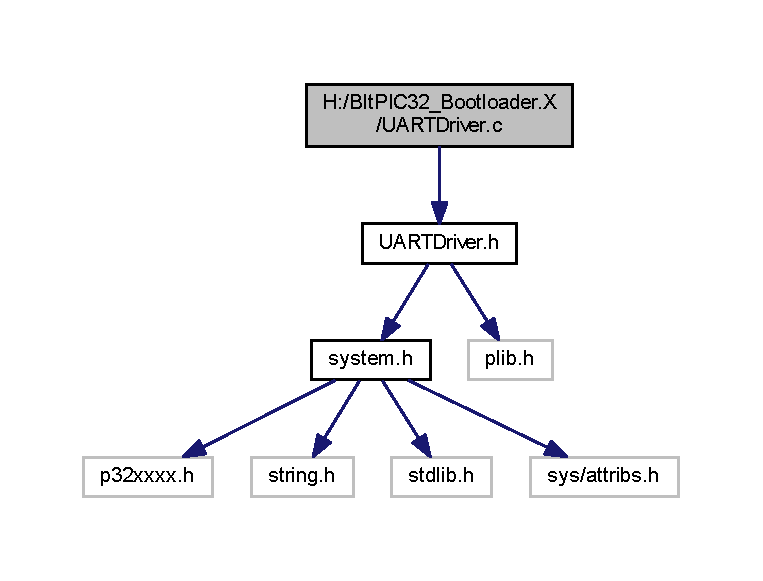
\includegraphics[width=332pt]{_u_a_r_t_driver_8c__incl}
\end{center}
\end{figure}
\subsection*{Functions}
\begin{DoxyCompactItemize}
\item 
\mbox{\Hypertarget{_u_a_r_t_driver_8c_a381c21700dd763626b378de6cb725317}\label{_u_a_r_t_driver_8c_a381c21700dd763626b378de6cb725317}} 
void \hyperlink{_u_a_r_t_driver_8c_a381c21700dd763626b378de6cb725317}{driver\+Config\+\_\+\+\_\+\+U\+A\+RT} (void)
\begin{DoxyCompactList}\small\item\em function configures U\+S\+A\+RT peripheral. \end{DoxyCompactList}\item 
\mbox{\Hypertarget{_u_a_r_t_driver_8c_aa66e9ab50d44d5c68a57cfb3b7833557}\label{_u_a_r_t_driver_8c_aa66e9ab50d44d5c68a57cfb3b7833557}} 
void \hyperlink{_u_a_r_t_driver_8c_aa66e9ab50d44d5c68a57cfb3b7833557}{send\+Data\+\_\+\+\_\+\+U\+A\+RT} (\hyperlink{system_8h_aba7bc1797add20fe3efdf37ced1182c5}{uint8\+\_\+t} data)
\begin{DoxyCompactList}\small\item\em function sends data to the host. \end{DoxyCompactList}\end{DoxyCompactItemize}


\subsection{Detailed Description}
In this file the U\+A\+RT config, send\+Data, I\+SR functions are defined. 

\begin{DoxyAuthor}{Author}
Mallikarjun Tirlapur 
\end{DoxyAuthor}
\begin{DoxyDate}{Date}
14 May, 2016, 11\+:38 PM 
\end{DoxyDate}

\hypertarget{_u_a_r_t_driver_8h}{}\section{H\+:/\+Blt\+P\+I\+C32\+\_\+\+Bootloader.X/\+U\+A\+R\+T\+Driver.h File Reference}
\label{_u_a_r_t_driver_8h}\index{H\+:/\+Blt\+P\+I\+C32\+\_\+\+Bootloader.\+X/\+U\+A\+R\+T\+Driver.\+h@{H\+:/\+Blt\+P\+I\+C32\+\_\+\+Bootloader.\+X/\+U\+A\+R\+T\+Driver.\+h}}


File contains the declaration of U\+A\+RT functions and uart\+\_\+rxbuffer array.  


{\ttfamily \#include \char`\"{}system.\+h\char`\"{}}\newline
{\ttfamily \#include \char`\"{}plib.\+h\char`\"{}}\newline
Include dependency graph for U\+A\+R\+T\+Driver.\+h\+:
\nopagebreak
\begin{figure}[H]
\begin{center}
\leavevmode
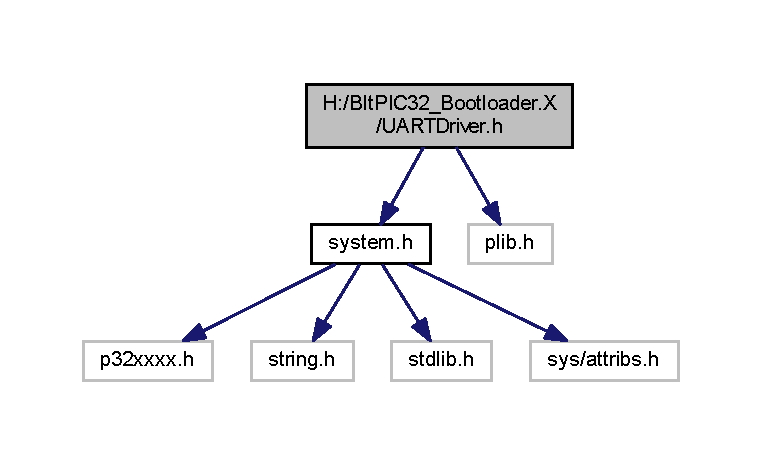
\includegraphics[width=350pt]{_u_a_r_t_driver_8h__incl}
\end{center}
\end{figure}
This graph shows which files directly or indirectly include this file\+:
\nopagebreak
\begin{figure}[H]
\begin{center}
\leavevmode
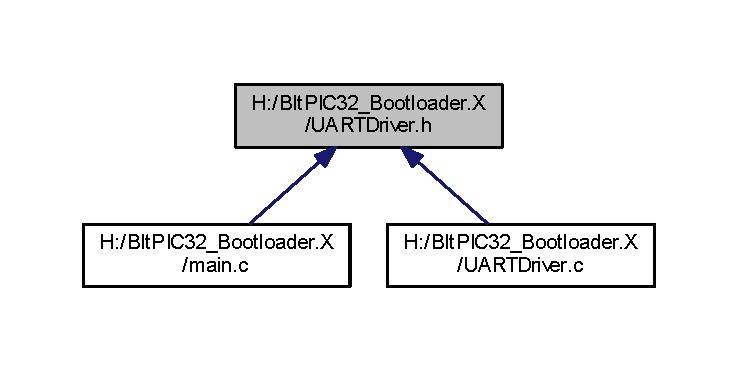
\includegraphics[width=350pt]{_u_a_r_t_driver_8h__dep__incl}
\end{center}
\end{figure}
\subsection*{Macros}
\begin{DoxyCompactItemize}
\item 
\hypertarget{_u_a_r_t_driver_8h_a7d5ce7b79462bbfb630ee53075540b65}{}\label{_u_a_r_t_driver_8h_a7d5ce7b79462bbfb630ee53075540b65} 
\#define {\bfseries S\+Y\+S\+\_\+\+F\+R\+EQ}~(40000000ul)
\item 
\hypertarget{_u_a_r_t_driver_8h_a734bbab06e1a9fd2e5522db0221ff6e3}{}\label{_u_a_r_t_driver_8h_a734bbab06e1a9fd2e5522db0221ff6e3} 
\#define {\bfseries B\+A\+U\+D\+R\+A\+TE}~(115200ul)
\end{DoxyCompactItemize}
\subsection*{Functions}
\begin{DoxyCompactItemize}
\item 
\hypertarget{_u_a_r_t_driver_8h_a381c21700dd763626b378de6cb725317}{}\label{_u_a_r_t_driver_8h_a381c21700dd763626b378de6cb725317} 
void \hyperlink{_u_a_r_t_driver_8h_a381c21700dd763626b378de6cb725317}{driver\+Config\+\_\+\+\_\+\+U\+A\+RT} (void)
\begin{DoxyCompactList}\small\item\em function configures U\+A\+RT peripheral. \end{DoxyCompactList}\item 
\hypertarget{_u_a_r_t_driver_8h_aa66e9ab50d44d5c68a57cfb3b7833557}{}\label{_u_a_r_t_driver_8h_aa66e9ab50d44d5c68a57cfb3b7833557} 
void \hyperlink{_u_a_r_t_driver_8h_aa66e9ab50d44d5c68a57cfb3b7833557}{send\+Data\+\_\+\+\_\+\+U\+A\+RT} (uint8\+\_\+t data)
\begin{DoxyCompactList}\small\item\em function sends data to the host. \end{DoxyCompactList}\end{DoxyCompactItemize}
\subsection*{Variables}
\begin{DoxyCompactItemize}
\item 
\hypertarget{_u_a_r_t_driver_8h_a130e6ee9d4b6aa42ac13165417f9c749}{}\label{_u_a_r_t_driver_8h_a130e6ee9d4b6aa42ac13165417f9c749} 
uint8\+\_\+t {\bfseries uart\+\_\+rxbuffer} \mbox{[}B\+Y\+T\+E\+\_\+\+R\+O\+W\+\_\+\+S\+I\+ZE\mbox{]}
\item 
\hypertarget{_u_a_r_t_driver_8h_a816e5f0aa1205d134039dbfa37338882}{}\label{_u_a_r_t_driver_8h_a816e5f0aa1205d134039dbfa37338882} 
uint8\+\_\+t {\bfseries uart\+\_\+rxbuffer\+\_\+counter}
\end{DoxyCompactItemize}


\subsection{Detailed Description}
File contains the declaration of U\+A\+RT functions and uart\+\_\+rxbuffer array. 

\begin{DoxyAuthor}{Author}
Mallikarjun Tirlapur 
\end{DoxyAuthor}
\begin{DoxyDate}{Date}
14 May, 2016 
\end{DoxyDate}

%--- End generated contents ---

% Index
\backmatter
\newpage
\phantomsection
\clearemptydoublepage
\addcontentsline{toc}{chapter}{Index}
\printindex

\end{document}
